\chapter{图模型}
\section{贝叶斯网}
\subsection{重要基本概念}
\subsubsection{马尔科夫网}
马尔科夫网用于描述边的独立性结构,形如“给定某某变量的值,其它变量相互独立”:$X\perp Y|Z$.核心就是条件概率分解.如下图:

\begin{center}
	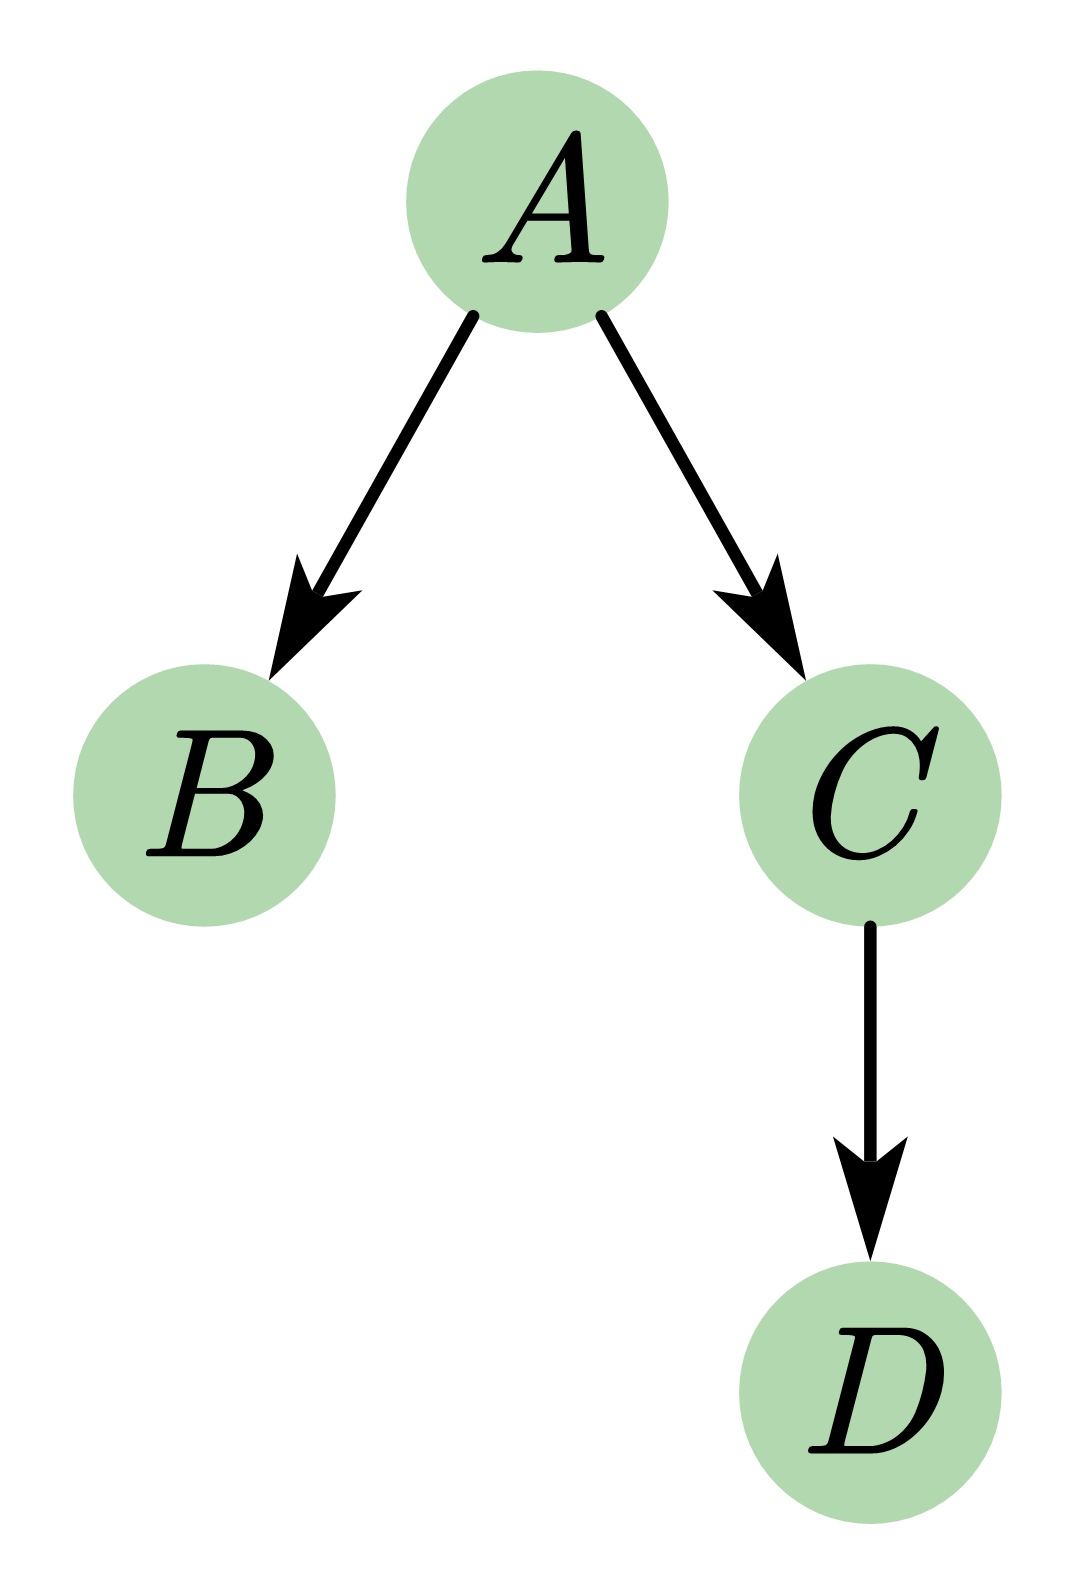
\includegraphics[width=3cm]{figure/BayesNet1.png}
\end{center}

表示概率分解:
\begin{empheq}{align*}
	P(A,B,C,D)&=P(A)P(B,C,D|A)\\
	&=P(A)P(B|A)P(C,D|A)\\
	&=P(A)P(B|A)P(D|C)P(C|A)\\
\end{empheq}

\subsubsection{等价类}
一个马尔科夫网的等价类是指:\circled{1}骨架相同;\circled{2}非正规结构(V结构)相同.骨架是指不考虑边的方向得到的边集.V结构形如:$X\rightarrow Z\leftarrow Y$,即双因.由于$Z$是由两个原因共同导致的,假如确定了$Z$,$X,Y$并不是独立,只有在某些情况下,才能共同诱导$Z$的特定值.

\subsubsection{do操作}
$\doop$也叫干预查询.图结构如下所示:
\begin{center}
	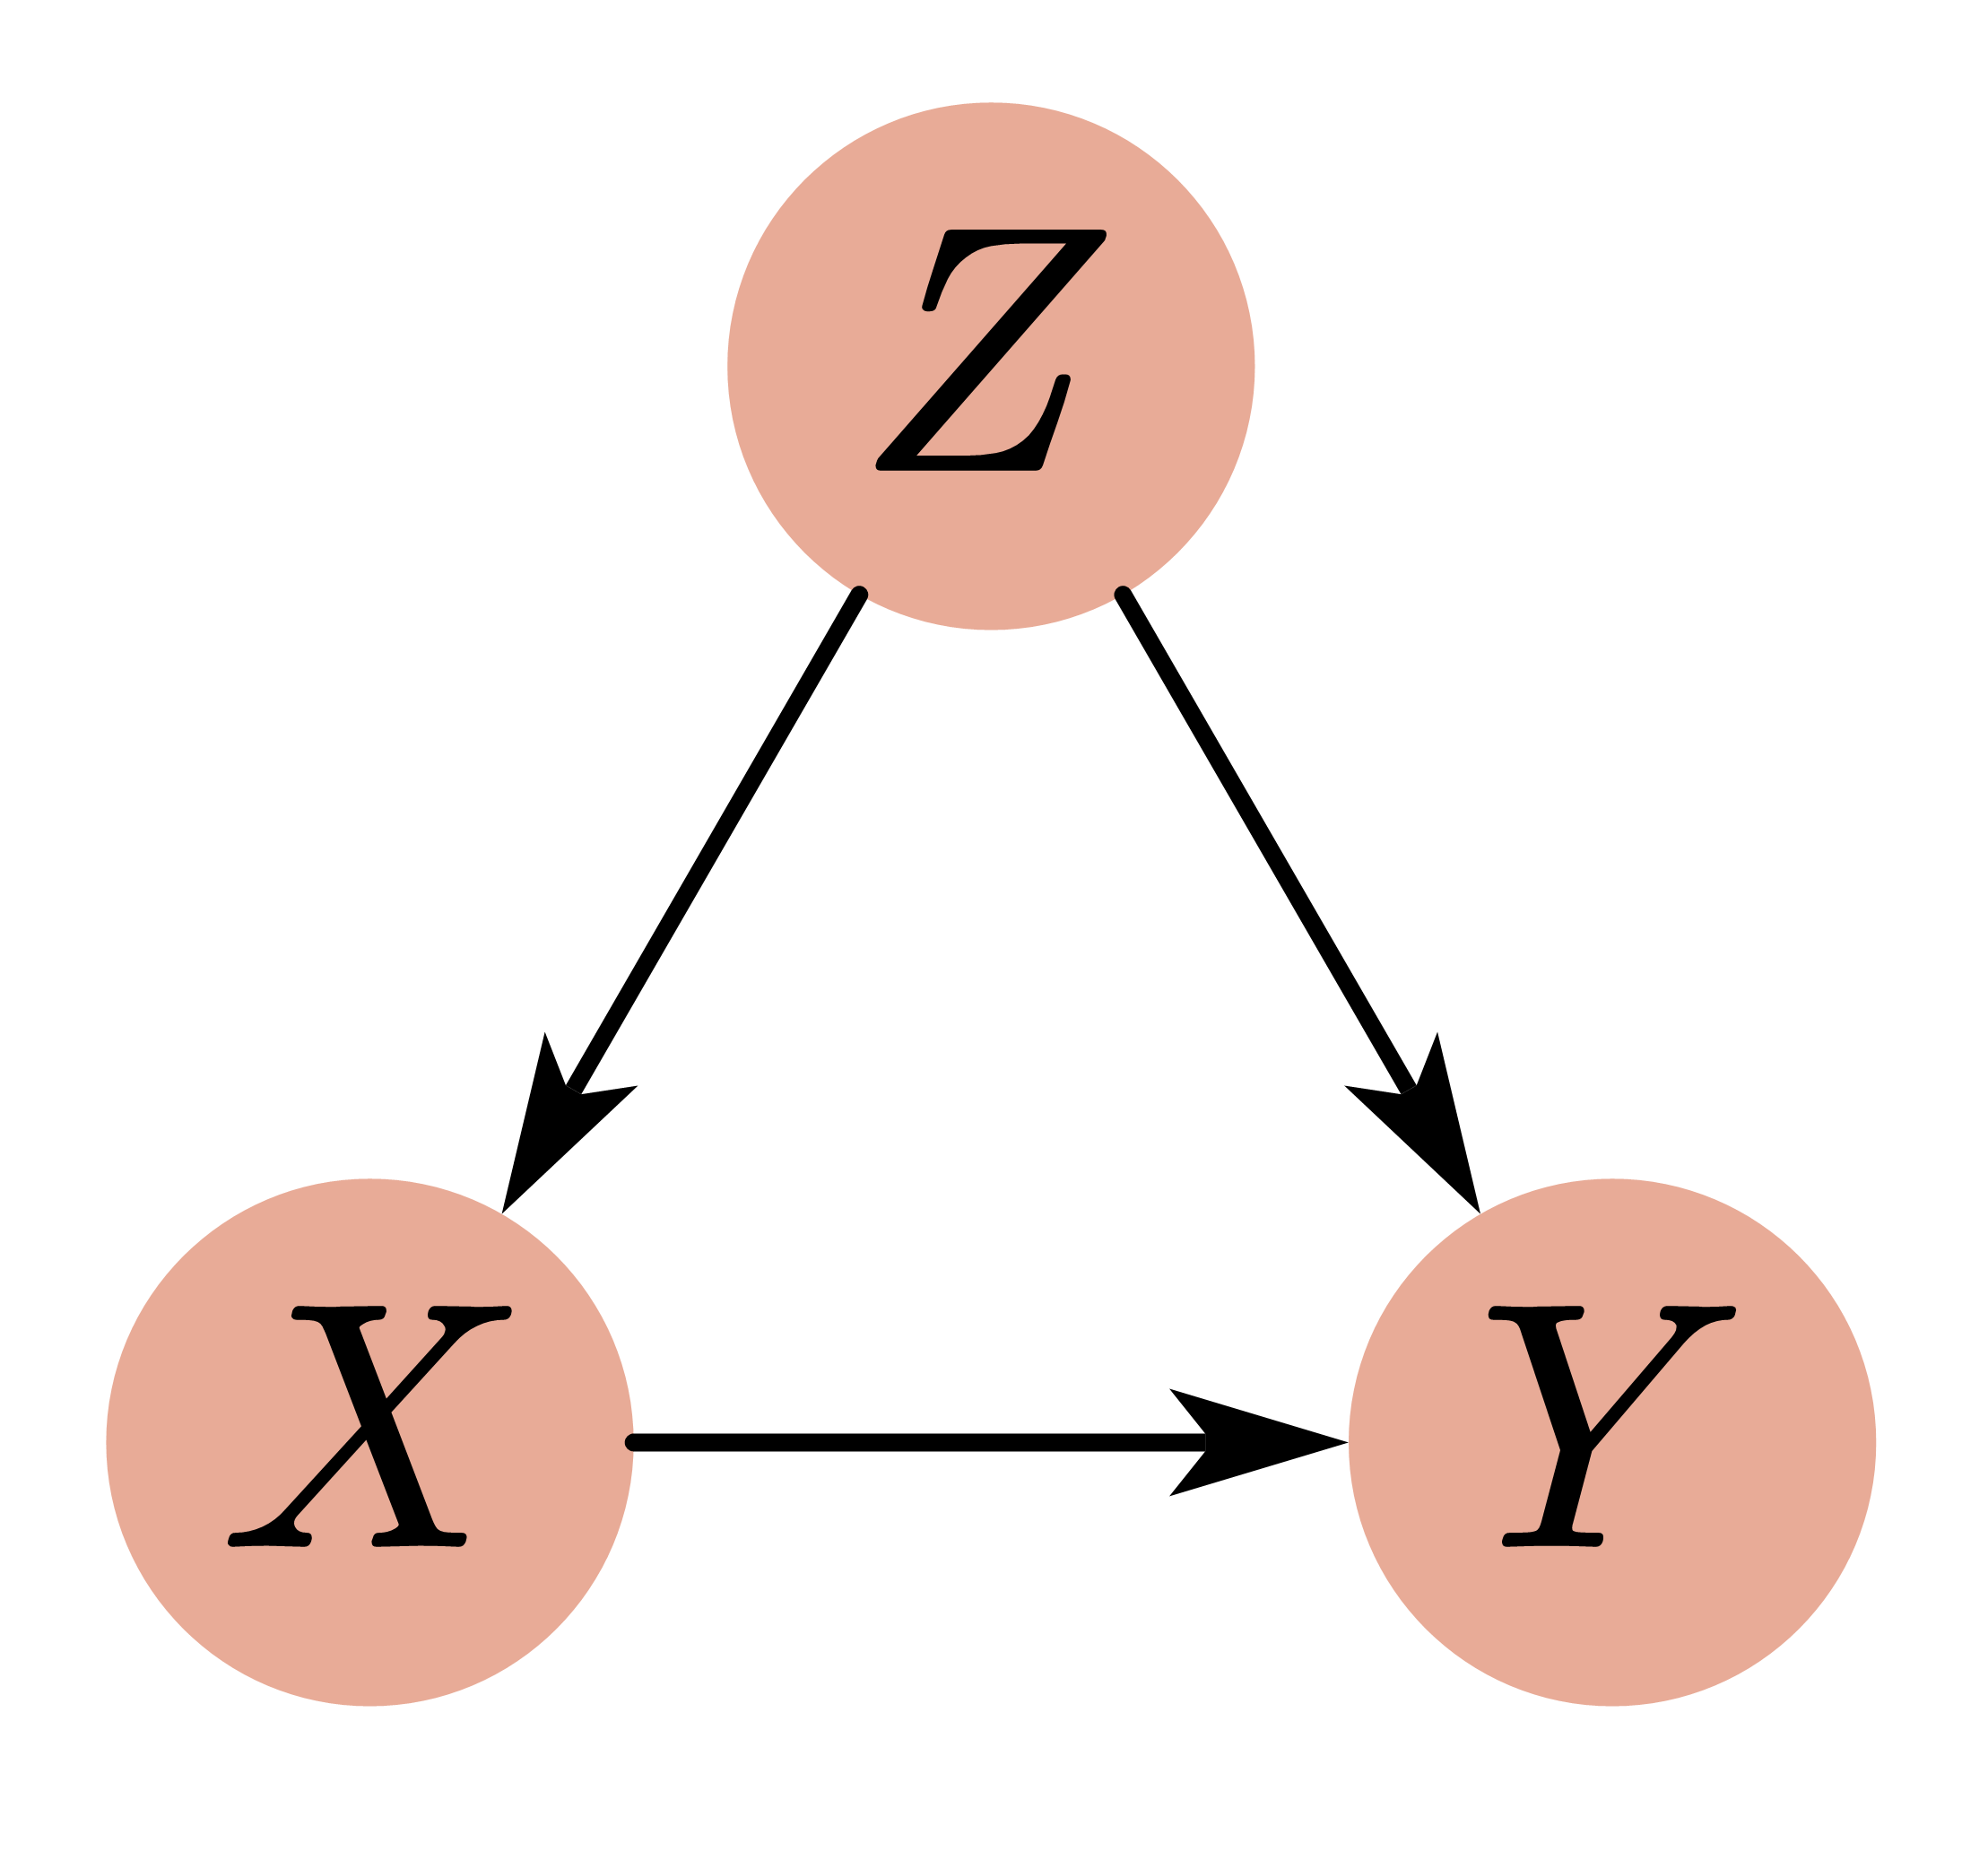
\includegraphics[width=3cm]{figure/Cofounder.png}
	\captionof{figure}{三变量网络}
	\label{fig:p5f1}
\end{center}

如果直接计算条件概率
\begin{empheq}{align*}
	\Prob(Y=y|X=x)&=\frac{\Prob(Y=y,X=x)}{\Prob(X=x)}\\
	&=\frac{\sum_z \Prob(Y=y,X=x|Z=z)\Prob(Z=z) }{\Prob(X=x)}\\
	&=\frac{\sum_z \Prob(Y=y|X=x,Z=z)\Prob(X=x|Z=z)P(Z=z) }{\Prob(X=x)}\\
	&=\frac{\sum_z \Prob(Y=y|X=x,Z=z)\Prob(X=x,Z=z) }{\Prob(X=x)}\\
	&=\sum_z \Prob(Y=y|X=x,Z=z)\Prob(Z=z|X=x)\label{condprob}
\end{empheq}

原本变量$X$由$Z$驱动,但使用$\doop X=x$操作后,$Z$就无法再影响$X$了,所以现在的图应当是
\begin{center}
	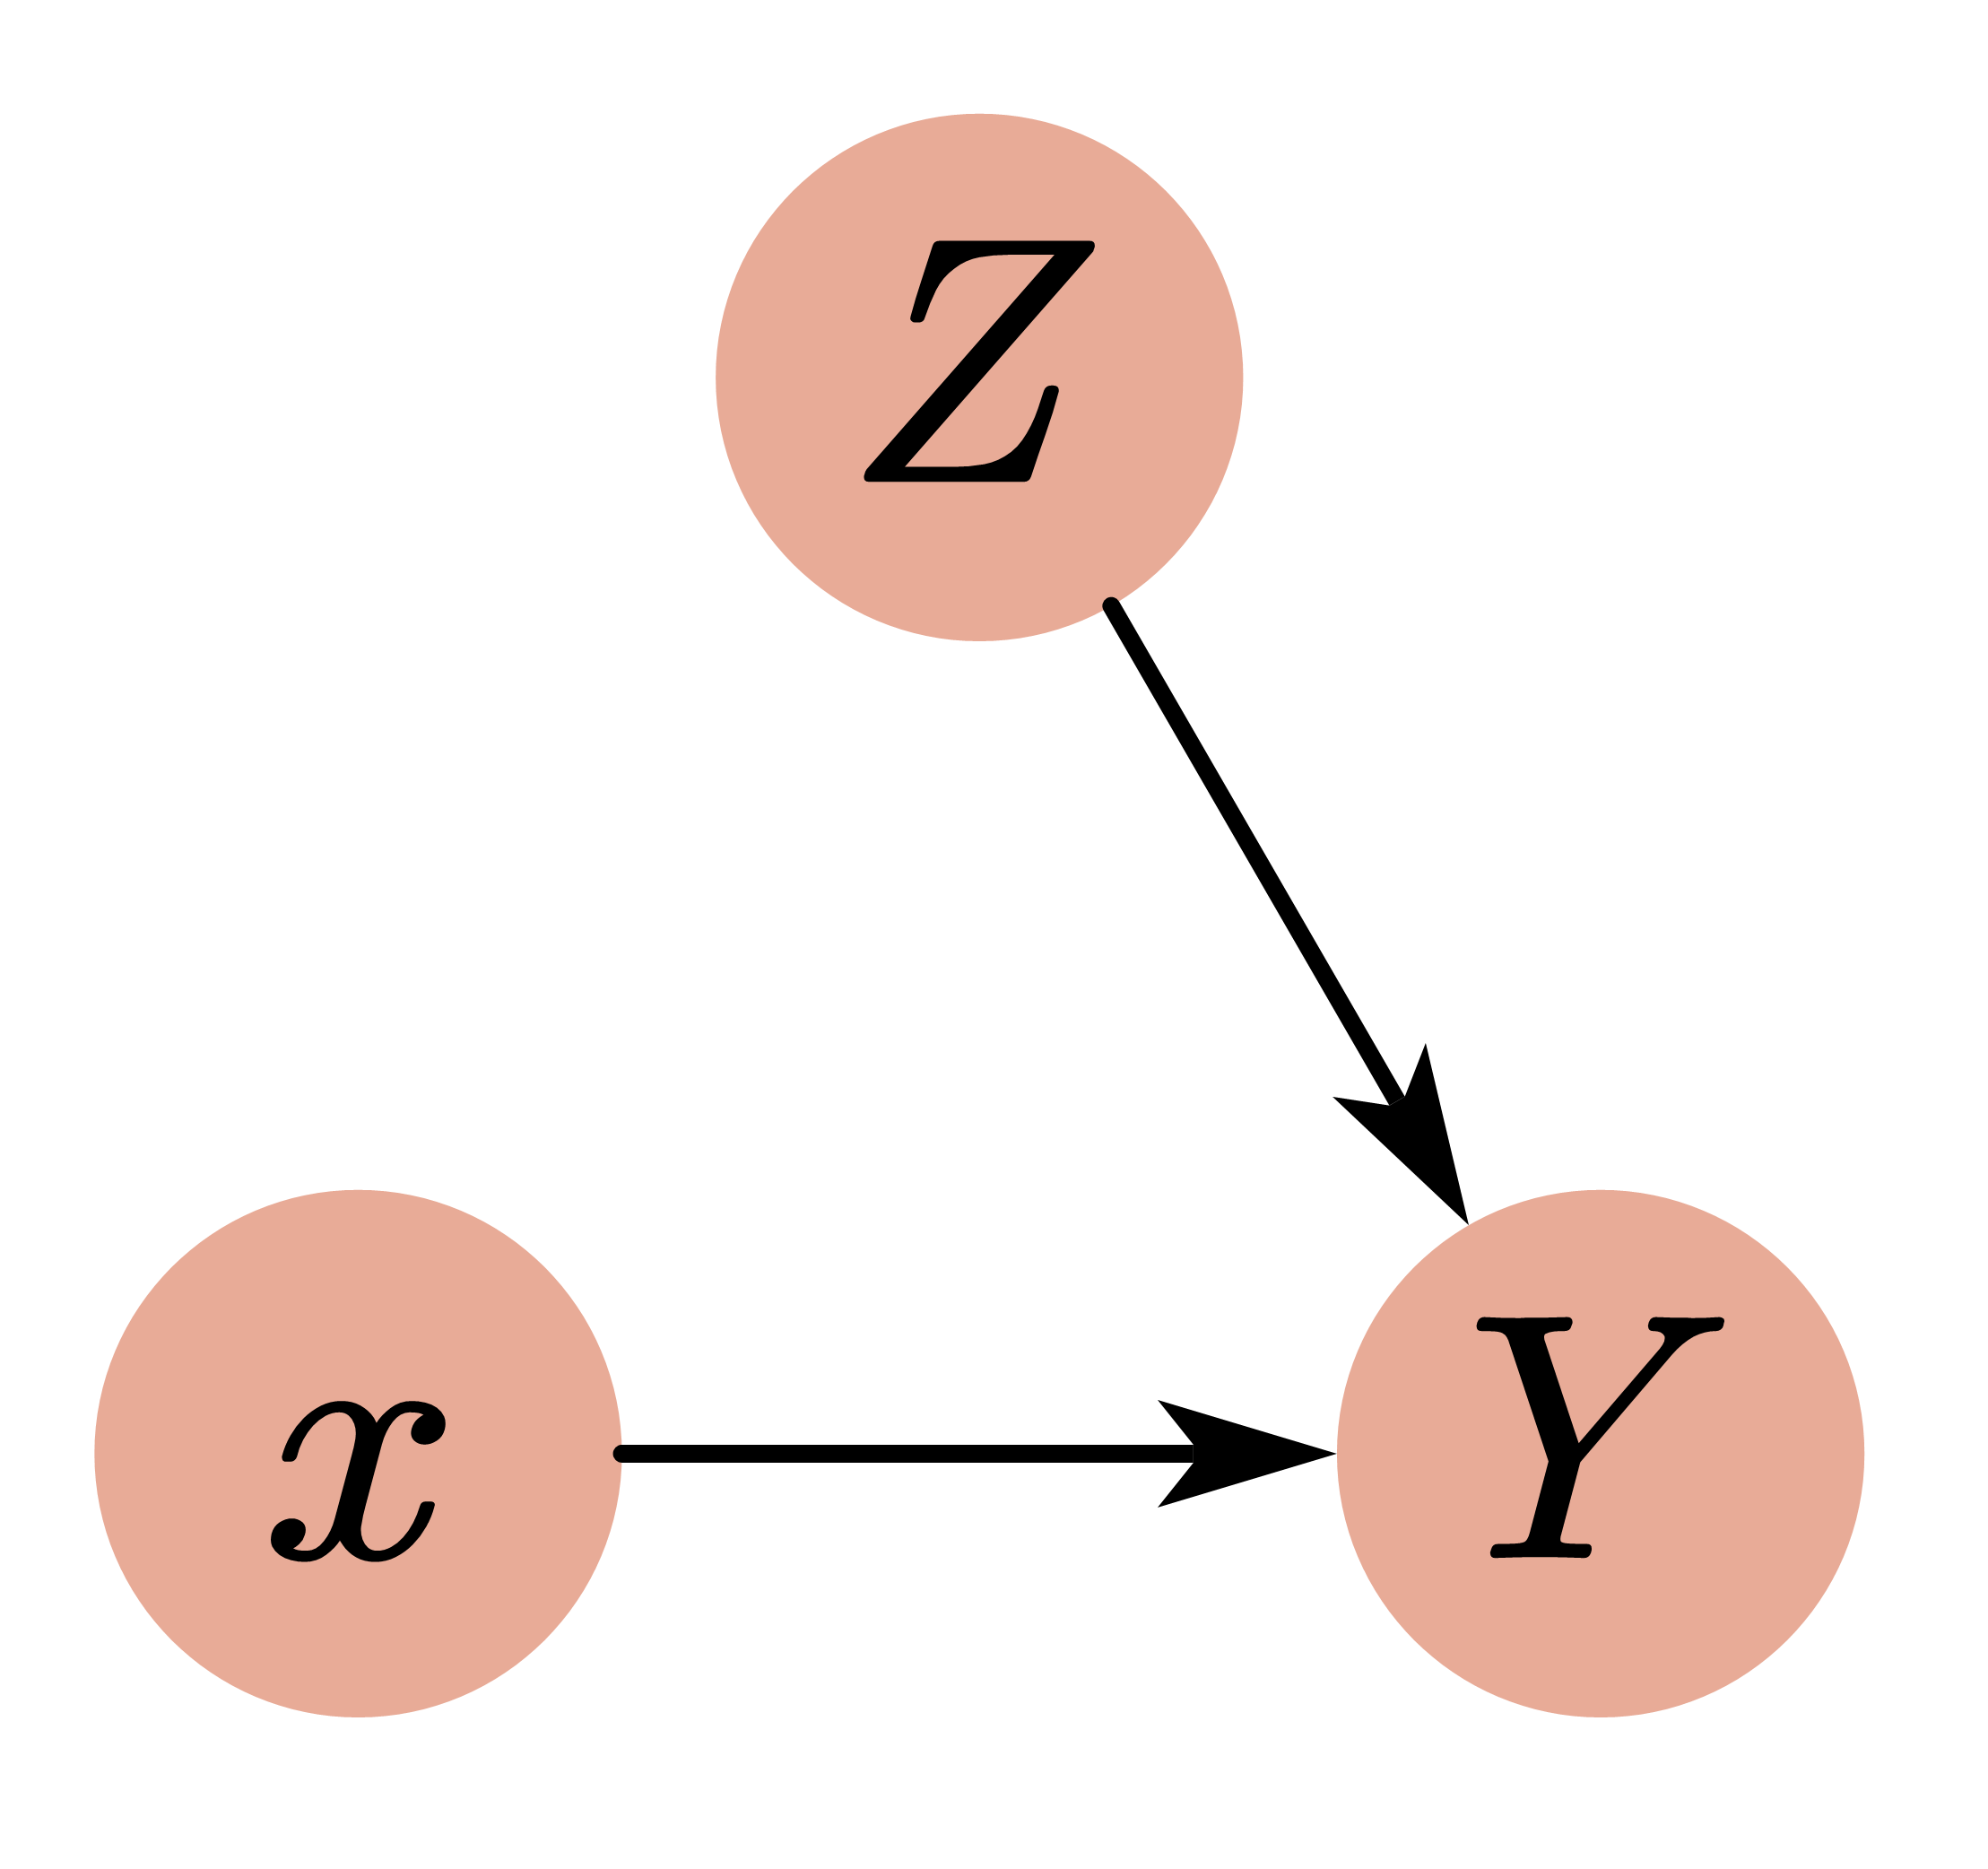
\includegraphics[width=3cm]{figure/bivar.png}
\end{center}
上图中$x$表示$X=x$,注意它现在已经不再是随机变量了,一下可以看出
\begin{empheq}{align}
	\Prob(Y=y|\doop X=x)&=\sum_z\Prob(Y=y|X=x,Z=z)\Prob(Z=z)\label{doprob}
\end{empheq}

之所以可以一步这样写,是因为$x$不是随机变量,而是类似于参数,假如暂时忽略它,那么就是
\begin{empheq}{align*}
	\Prob(Y=y)&=\sum_z\Prob(Y=y|Z=z)\Prob(Z=z)
\end{empheq}

现在把参数$x$加进去,就可以得到\eqref{doprob}.

以上可以看出,$\doop$操作的实质就是阻断因果关系.

另一方面,使用$\doop$后,$X$仍然可以理解为随机变量,但现在$\Prob(X=x)=1$,把这个条件加入\eqref{condprob}中,可以得到
\begin{empheq}{align*}
	\Prob(Y=y|X=x)
	&=\sum_z \Prob(Y=y|X=x,Z=z)\Prob(Z=z|X=x)\\
	\xRightarrow{P(X=x)=1}&\sum_z \Prob(Y=y|X=x,Z=z)\Prob(Z=z|1)\\
	&=\sum_z \Prob(Y=y|X=x,Z=z)\Prob(Z=z)\\
	\implies&\Prob(Y=y|\doop X=x)
\end{empheq}

这样我们从两个角度理解了$\doop$操作的实质.
\subsection{推理与计算}


\subsubsection{}
